\section{les composantes d'un réseau IoT :}

Un système IoT réunit de nombreux acteurs et composants technologiques. Il est composé d'objets connectés, de réseaux de communication et de plateformes de services IoT pour les utilisateurs finaux.

\begin{figure}[h]
	\centering
    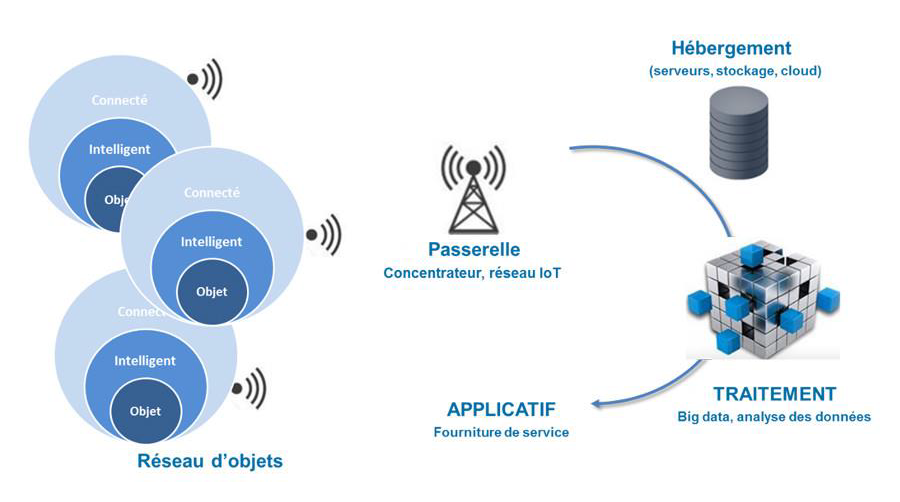
\includegraphics[scale=0.5]{img/part1/2.2}
    \caption{composantes d'un réseau IoT}
\end{figure}

\subsection{Les objets connecté:}
Les objets connectés sont des capteurs ou des objets dotés de capteurs capables de communiquer (envoyer et recevoir) des données à travers un réseau. Les données sont généralement envoyées à un ordinateur, une tablette, un smartphone ou tout autre appareil électronique et parfois via Internet pour que l’information soit accessible sur tous les appareils pouvant s’y connecter.

On distingue deux types d’objet :
\begin{itemize}[label=\textbullet]
\item \textbf{Les objets passifs :} ils utilisent généralement un tag (puce RFID, code barre 2D). Ils embarquent une faible capacité de stockage (de l’ordre du kilo-octet) leur permettant d’assurer un rôle . Ils peuvent parfois, dans le cas d’une puce RFID, embarquer un capteur (température, humidité) et être réinscriptibles.
\item \textbf{Les objets actifs :} ils peuvent être équipés de plusieurs de capteurs, d’une plus grande capacité de stockage, être doté d’une capacité de traitement ou encore être en mesure de communiquer sur un réseau.
\end{itemize}

\newpage 
\subsubsection{Exemples d’objets connectés}
Voici quelques objets connectés :
\begin{figure}[h]
	\centering
    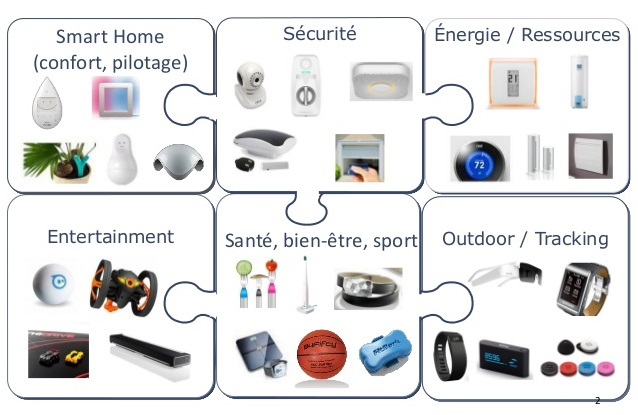
\includegraphics[scale=0.5]{img/part1/2.3}
    \caption{Exemples d’objets connectés}
\end{figure}
Comme on peut le voir on en retrouve de toute sorte : des appareils électroménagers comme les fours, les réfrigérateurs qui ont une capacité de se connecter à internet et de faciliter la vie des utilisateurs. Des camera connectée qui permettent aux utilisateurs via une application sur son Smartphone de vérifier en temps réel l'état de sa maison. Des Bracelets de santé connectés, des lunettes..etc

\subsubsection{Les composants d’un objet connecté :}
Les 4 composants essentiels, à la réalisation d’un objet connecté :
\begin{itemize}[label=\textbullet]
\item \textbf{Le capteur :} pour mesurer un paramètre extérieur tel qu’une température, un niveau d’humidité, un mouvement, un niveau de remplissage ou une pression atmosphérique… ou pour savoir si votre objet dysfonctionne, ou présente par exemple un défaut d’alimentation électrique. Tout débute par une prise d’information dans le monde physique. Bien sûr, l’objet peut intégrer plusieurs capteurs.

Il en existe de tout type: 
\begin{figure}[h]
	\centering
    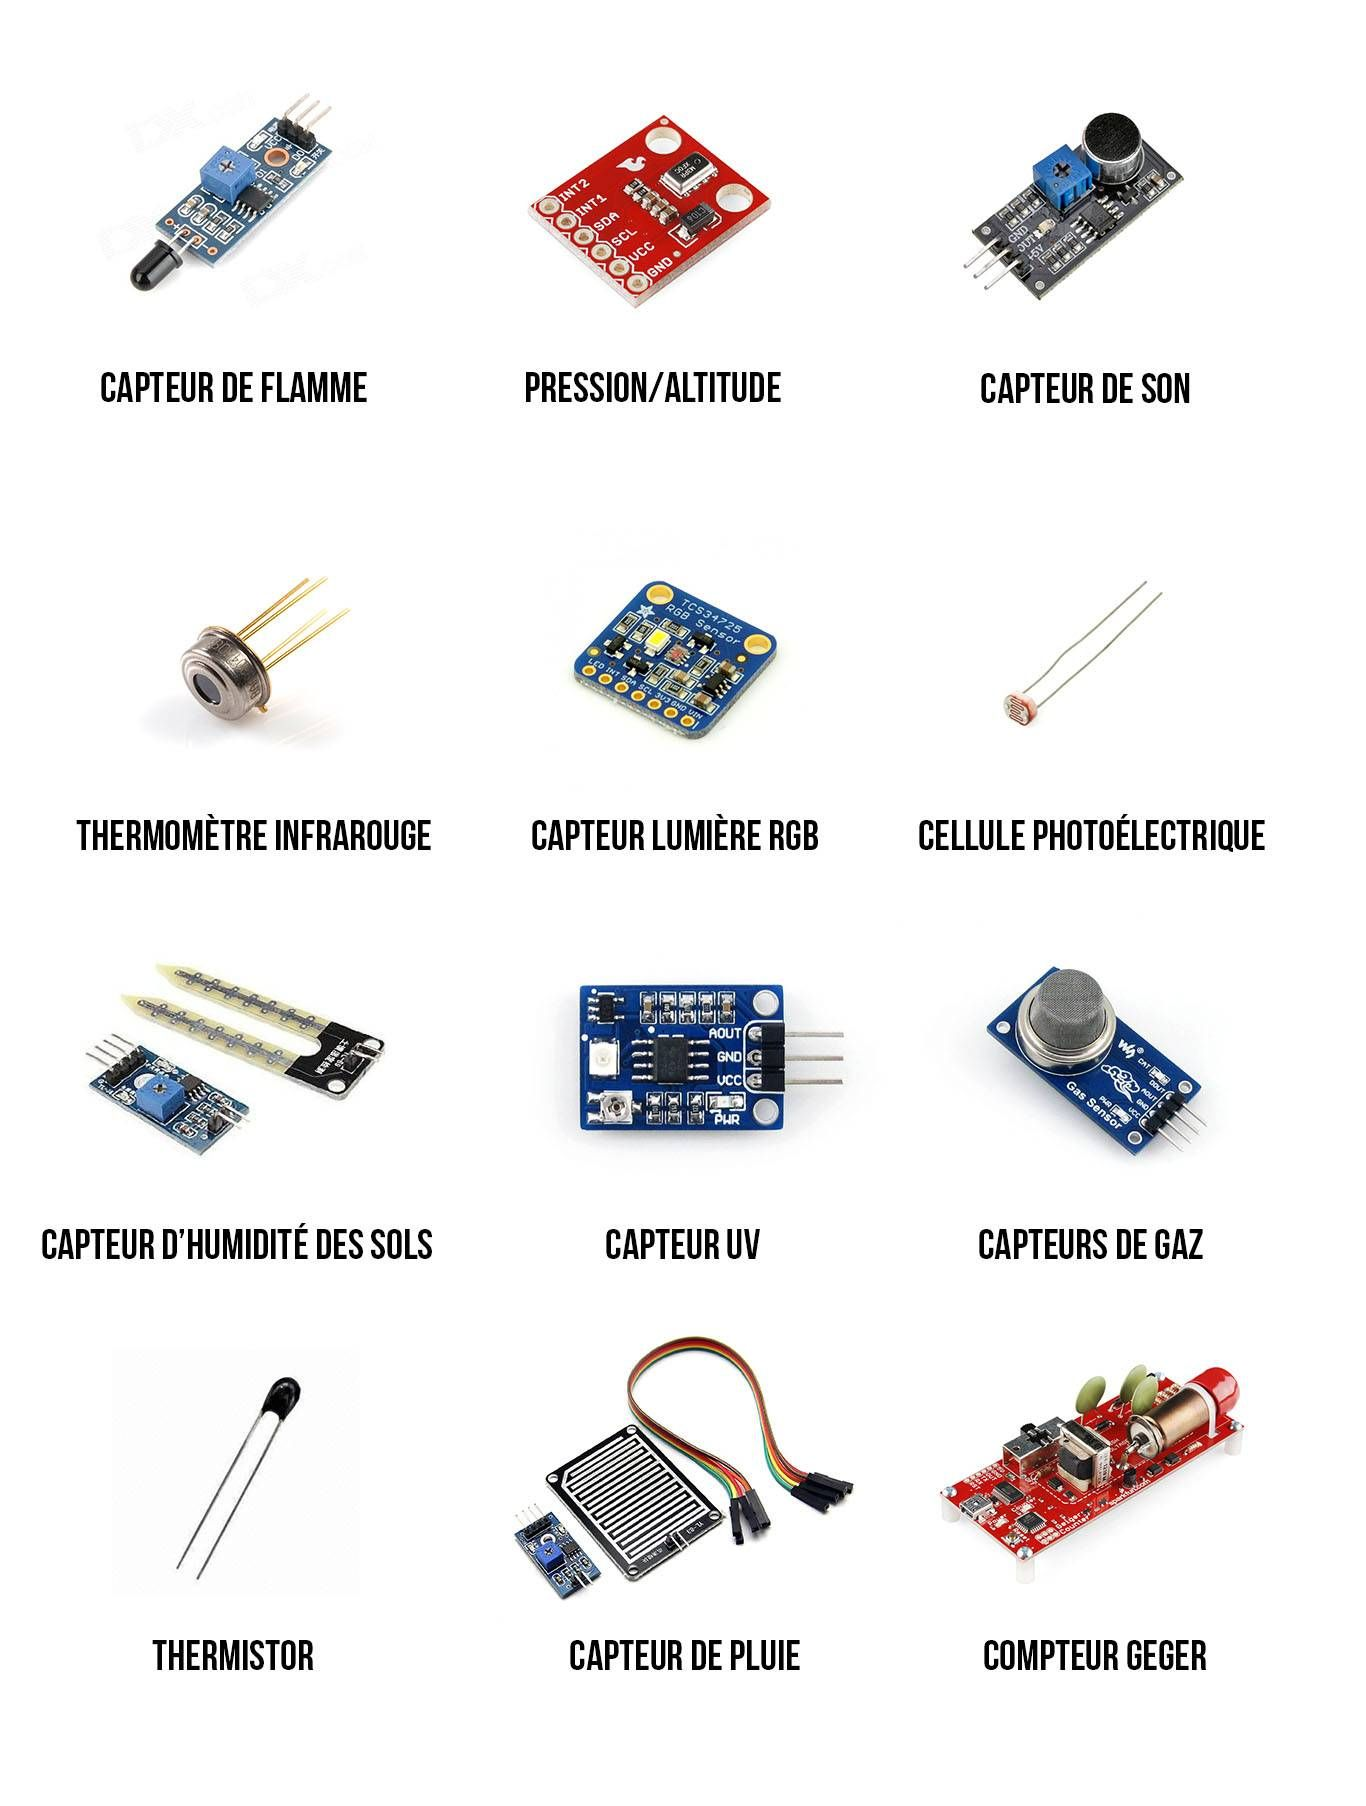
\includegraphics[scale=0.1]{img/part1/2.4}
    \caption{Exemples de capteurs}
\end{figure}

\item \textbf{Le logiciel embarqué :} Une fois l’information récupérée, il faut pouvoir stocker cette information et la traiter avant de la transmettre. C’est pour cela qu’on évoque parfois des objets « intelligents ». En effet, la plupart du temps, l’information est stockée localement, il s’agit d’attendre d’avoir plusieurs mesures successives ou de types différents et de les compiler pour pouvoir les transmettre.
\item \textbf{La puce de transmission :} lorsque l’information a été compilée, elle est prête à l’envoi. C’est à ce moment qu’intervient la puce de transmission. Celle-ci diffère en fonction du type de réseau, du volume d’informations à transmettre et de la vitesse de transfert.
\item \textbf{La batterie :} bien-sûr les objets connectés peuvent être alimentés par une prise électrique, mais la plupart du temps, ils sont autonomes. Dès lors, l’un des enjeux des ingénieurs est de réduire au maximum la dépense d’énergie des différents composants pour augmenter la durée de vie et/ou réduire la taille de l’objet. Le composant le plus énergivore est la puce de transmission. Ainsi, si votre objet transmet des informations à un rythme soutenu, vous risquez d’écourter sa durée de vie. C’est là qu’intervient l’intelligence embarquée permettant de ne transmettre que l’information pertinente et au moment où vous en avez besoin. De plus, les différents types de connectivité (Bluetooth, wifi, GSM, LPWA) ne sont pas équivalents en matière de consommation énergétique.
\end{itemize}

\subsection{Les réseaux de communication :}
Une fois capté, il est nécessaire de transporter la donnée vers internet. Ce transport peut se faire à l’aide de différents types de réseaux de communication. Ces réseaux seront utilisés en fonction du cas d’usage. Il faut donc choisir le réseau le plus adapté au cas d’usage requis car leur application va dépendre du débit souhaité. On peut alors les catégoriser en réseau haut débit ou bas débit.

Dans les réseaux hauts débits, on retrouve les réseaux habituels tels que les réseaux cellulaires (3G, 4G), Wifi et câblés (cuivre, fibre). En compléments, de nouveaux réseaux « bas débits » sont apparus depuis des années, donnant la possibilité à certains types d’objets d’être indépendant énergiquement et bénéficiant d’une longue portée de couverture radio. On les appelle les LPWAN – Low Power Wide Area Network. On retrouve notamment dans cette catégorie la technologie LoRa, déployée librement à l’échelle nationale par certains opérateurs , mais que l’on peut également déployer soi-même pour créer son propre réseau privé. Ce réseau permet une économie de la batterie des capteurs dans le but d’obtenir une autonomie de 2 à 10 ans et ainsi de réduire les coûts financiers de déploiement \& maintenance.

\begin{figure}[h]
	\centering
    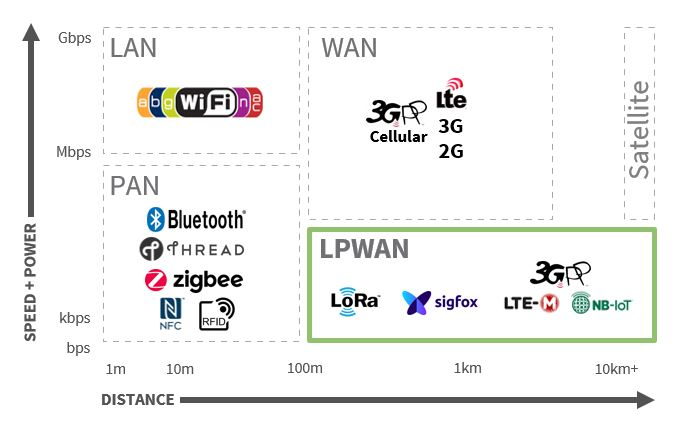
\includegraphics[scale=0.4]{img/part1/2.5}
    \caption{Réseaux de communication }
\end{figure}

\subsection{Les plateformes de service IoT:}
Après avoir créé et transmis la donnée, il faut l’analyser, la stocker et la restituer aux clients d’où la création d’une plateforme de services IoT. Certaines données sont directement exploitables tandis que d’autres nécessitent des « savoir-faire métier » pour transmettre des informations utiles et utilisables. Il existe donc deux types de plateformes sur le marché :
\begin{itemize}[label=\textbullet]
\item Les plateformes dites « verticales » vont traiter un cas d’usage spécifique très rapidement et proposent un ensemble de fonctionnalité (interface adaptée, notifications en temps réel, automatisation des rapports…). Par exemple, BH Technologies propose 2 solutions dans le but de gérer à distance l’éclairage public ainsi que la télérelève pour optimiser le ramassage des déchets au sein des villes.
\item Les plateformes dites « horizontales », génériques qui développent des applications sur mesure. Par exemple, la plateforme de NomoSense permet d’agréger des applications IoT de manière simple et ergonomique.
\end{itemize}

\begin{figure}[h]
	\centering
    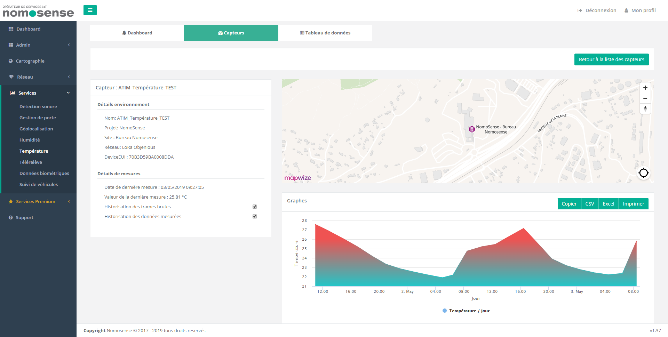
\includegraphics[scale=0.9]{img/part1/2.6}
    \caption{Les plateformes de service IoT}
\end{figure}